% Introducción
\chapter{Arquitectura} % Chapter title

\label{ch:arquitectura} % For referencing the chapter elsewhere, use \autoref{ch:introduccion} 

%----------------------------------------------------------------------------------------
\graffito{A cada uno de los servicios enunciados en este informe le corresponde una carpeta dentro del repositorio del proyecto. El código fuente solo es accesible por los colaboradores y se encuentra en \url{https://github.com/sebastianaf/pricecloud}.\bigskip}

\graffito{La primera parte del proyecto no comprende ningun aspecto de la interfaz gráfica, sin embargo fue necesario implementar el \emph{Login} que usará la aplicación para configurar el esquema básico de autenticación.\bigskip}

\graffito{Las credenciales del usuario administrador de la \acrshort{API} son: \textbf{usuario:} \emph{admin}, \textbf{contraseña:} \emph{price22cloud}.\bigskip}


\section{Esquema de servicios}
\begin{center}
    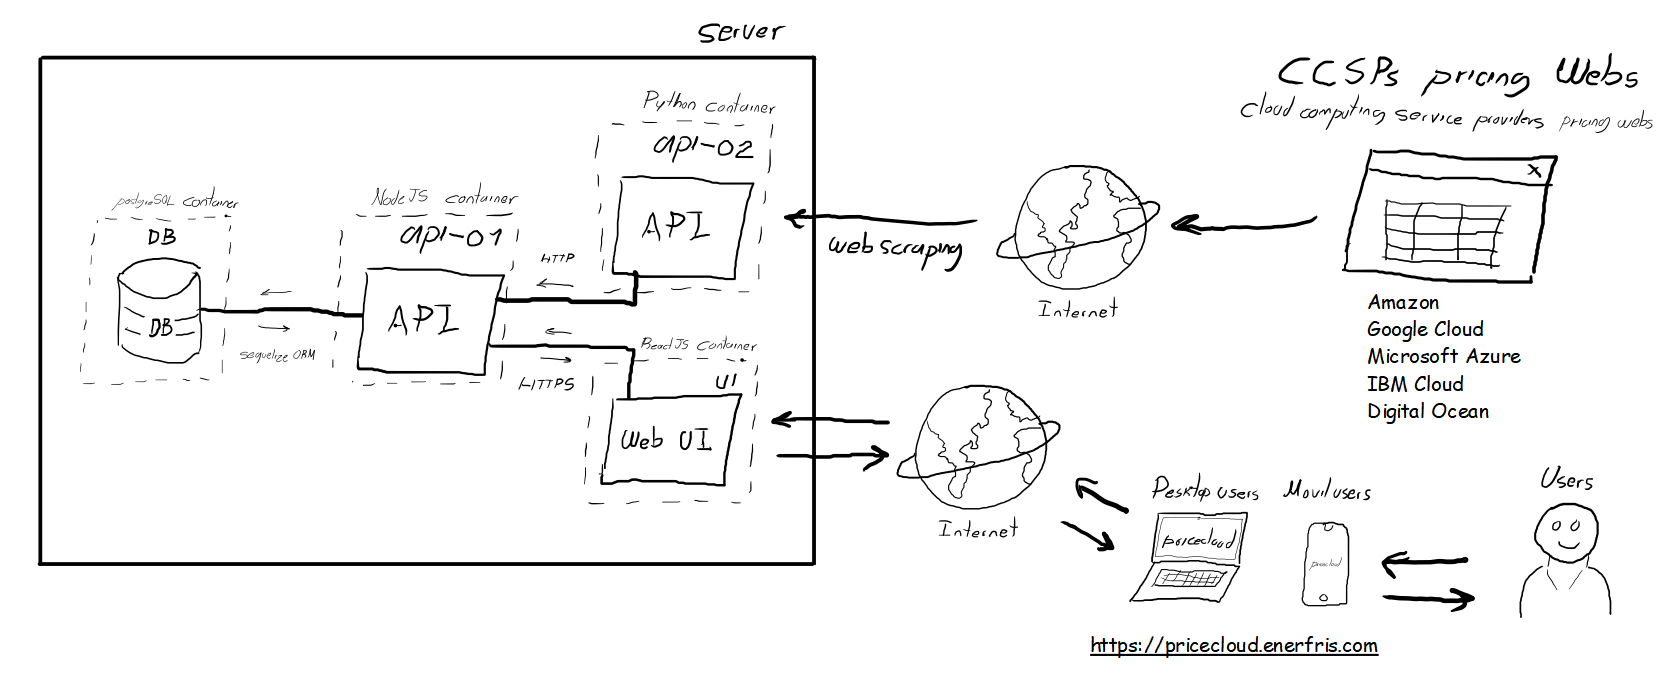
\includegraphics[width=\textwidth]{gfx/whiteSketch.png}
\end{center}

\section{Descripción de los servicios}
La primera parte del proyecto de grado atiende las actividades relacionadas con la etapa de \emph{Creación del modelo de evaluación de costos} y con las actividades relacionadas con la etapa de \emph{Creación del prototipo de microservicios de backend}. El servicio de backend está compuesto por tres microservicios con funciones específicas cada uno descritas acontinuación.

\subsection{\emph{api-01}}
El primer microservicio del backend se encarga de autenticar los usuarios de la aplicación y centralizar todas las peticiones. Este servicio está expuesto en Internet en la dirección \url{https://api.pricecloud.enerfris.com} se comunica usando el protocolo \acrfull{HTTPS} con el servicio de la interfaz web autenticando cada petición con \emph{JSON Web Tokens} cifrados con \acrfull{AES}; La responsabilidad de este servicio es responder todas las peticiones creadas por el frontend de la aplicación incluyendo las consultas de los precios de los \acrfullpl{CCSP} almacenadas en la base de datos.

\subsection{\emph{api-02}}
El segundo microservicio de backend se encarga de recopilar la información de precios de los \acrshortpl{CCSP}. Usando técnicas de \emph{Web Scraping} periodicamente es invocado por \emph{api-01} cual se encarga de recibir la información y gestionar su almacenamiento en la base de datos, este microservicio se basa en \gls{XPath} sobre \emph{Python}.

\subsection{\emph{db}}
Finalmente el último microservicio del backend corresponde a la base de datos. En el respositorio del proyecto no existe mas código relacionado con este servicio que el implementado por el \emph{script de despliegue} en el archivo \emph{docker-compose.yml} esto se debe a que todo el esquema de la base de datos reside en \emph{api-01} definido por \gls{Sequelize}.

\subsection{\emph{ui}}
Este servicio se encarga de ejecutar el servidor web con la interfaz de usuario. Implementa el esquema básico de autenticación que se usará en el resto de la aplicación con \emph{api-01} enviando un \emph{token} en las \emph{headers} peticiones \acrshortpl{HTTPS}.
